
%%\documentclass[12pt,preprint]{aastex}

%% manuscript produces a one-column, double-spaced document:

%% \documentclass[10pt,manuscript]{aastex}

%% preprint2 produces a double-column, single-spaced document:
\documentclass[preprint2,iop,numberedappendix,twocolappendix,appendixfloats]{emulateapj}
%% \documentclass[preprint2,iop]{aastex}

%% \documentclass[preprint2,longabstract]{aastex}

%% \usepackage{ccaption}
%% \captionstyle{\raggedright}
\usepackage[caption=false]{subfig}
\usepackage{amsmath}
\usepackage{footnote}
\bibpunct{(}{)}{;}{a}{}{,} 
\captionsetup{belowskip=12pt,aboveskip=4pt}
\setlength{\textfloatsep}{10pt plus 1.0pt minus 2.0pt}
\newcommand{\dif}{\mathrm{d}}
%% \renewcommand*{\thefootnote}{\fnsymbol{footnote}}

\def\nar{{New~A~Rev.}}          % New Astronomy Review
\def\pasa{{PASA}}               % Publications of the Astron. Soc. of Australia

%% \bibliographystyle{mn2e}
%% \bibliographystyle{apj}

\shorttitle{Estimate of Foregrounds in EoR Power Spectra for HERA}
\shortauthors{Thyagarajan et~al.}

\def\ASU{\altaffilmark{1}}
\def\ASUtxt{\altaffiltext{1}{Arizona State University, School of Earth and Space Exploration, Tempe, AZ 85287, USA}}

\def\myemail{\altaffilmark{*}}
\def\myemailtxt{\altaffiltext{*}{e-mail: t\_nithyanandan@asu.edu}}

\def\UW{\altaffilmark{2}}
\def\UWtxt{\altaffiltext{2}{University of Washington, Department of Physics, Seattle, WA 98195, USA}}

\def\SKASA{\altaffilmark{3}}
\def\SKASAtxt{\altaffiltext{3}{Square Kilometre Array South Africa (SKA SA), Park Road, Pinelands 7405, South Africa}}

\def\RU{\altaffilmark{4}}
\def\RUtxt{\altaffiltext{4}{Department of Physics and Electronics, Rhodes University, Grahamstown 6140, South Africa}}

\def\CfA{\altaffilmark{5}}
\def\CfAtxt{\altaffiltext{5}{Harvard-Smithsonian Center for Astrophysics, Cambridge, MA 02138, USA}}

\def\ANU{\altaffilmark{6}}
\def\ANUtxt{\altaffiltext{6}{Australian National University, Research School of Astronomy and Astrophysics, Canberra, ACT 2611, Australia}}

\def\CAASTRO{\altaffilmark{7}}
\def\CAASTROtxt{\altaffiltext{7}{ARC Centre of Excellence for All-sky Astrophysics (CAASTRO)}}

\def\Haystack{\altaffilmark{8}}
\def\Haystacktxt{\altaffiltext{8}{MIT Haystack Observatory, Westford, MA 01886, USA}}

\def\MIT{\altaffilmark{9}}
\def\MITtxt{\altaffiltext{9}{MIT Kavli Institute for Astrophysics and Space Research, Cambridge, MA 02139, USA}}

\def\Curtin{\altaffilmark{10}}
\def\Curtintxt{\altaffiltext{10}{International Centre for Radio Astronomy Research, Curtin University, Perth, WA 6845, Australia}}

\def\Victoria{\altaffilmark{11}}
\def\Victoriatxt{\altaffiltext{11}{Victoria University of Wellington, School of Chemical \& Physical Sciences, Wellington 6140, New Zealand}}

\def\UWisc{\altaffilmark{12}}
\def\UWisctxt{\altaffiltext{12}{University of Wisconsin--Milwaukee, Department of Physics, Milwaukee, WI 53201, USA}}

\def\UMichigan{\altaffilmark{13}}
\def\UMichigantxt{\altaffiltext{13}{University of Michigan, Department of Atmospheric, Oceanic and Space Sciences, Ann Arbor, MI 48109, USA}}

\def\UMelbourne{\altaffilmark{14}}
\def\UMelbournetxt{\altaffiltext{14}{The University of Melbourne, School of Physics, Parkville, VIC 3010, Australia}}

\def\USydney{\altaffilmark{15}}
\def\USydneytxt{\altaffiltext{15}{The University of Sydney, Sydney Institute for Astronomy, School of Physics, NSW 2006, Australia}}

\def\CASS{\altaffilmark{16}}
\def\CASStxt{\altaffiltext{16}{CSIRO Astronomy and Space Science (CASS), PO Box 76, Epping, NSW 1710, Australia}}

\def\Tata{\altaffilmark{17}}
\def\Tatatxt{\altaffiltext{17}{National Centre for Radio Astrophysics, Tata Institute for Fundamental Research, Pune 411007, India}}

\def\RRI{\altaffilmark{18}}
\def\RRItxt{\altaffiltext{18}{Raman Research Institute, Bangalore 560080, India}}

\def\NRAO{\altaffilmark{19}}
\def\NRAOtxt{\altaffiltext{19}{National Radio Astronomy Observatory, Charlottesville and Greenbank, USA}}

\def\UWA{\altaffilmark{20}}
\def\UWAtxt{\altaffiltext{20}{International Centre for Radio Astronomy Research, University of Western Australia, Crawley, WA 6009, Australia}}

%% \definenote[thanks][conversion=set 2]

\begin{document}

\title{Estimation of Foregrounds in Wide-Field Measurements of Redshifted 21~cm Power Spectra with the Hydrogen Epoch of Reionization Array}

%% Use \author, \affil, and the \and command to format
%% author and affiliation information.
%% Note that \email has replaced the old \authoremail command
%% from AASTeX v4.0. You can use \email to mark an email address
%% anywhere in the paper, not just in the front matter.
%% As in the title, use \\ to force line breaks.

%% Author list
\author{
%% Lead Authors
Nithyanandan~Thyagarajan\ASU\myemail,
TBD
% Daniel~C.~Jacobs\ASU,
% Judd~D.~Bowman\ASU,
% N.~Barry\UW,
% A.~P.~Beardsley\UW,
% G.~Bernardi\SKASA$^,$\RU$^,$\CfA,
% F.~Briggs\ANU$^,$\CAASTRO,
% R.~J.~Cappallo\Haystack, 
% P.~Carroll\UW,
% B.~E.~Corey\Haystack, 
% % A.~A.~Deshpande\RRI, 
% A.~de~Oliveira-Costa\MIT,
% Joshua~S.~Dillon\MIT,
% D.~Emrich\Curtin,
% % B.~M.~Gaensler\USydney$^,$\CAASTRO, 
% A.~Ewall-Wice\MIT,
% L.~Feng\MIT,
% R.~Goeke\MIT,
% L.~J.~Greenhill\CfA,
% B.~J.~Hazelton\UW, 
% J.~N.~Hewitt\MIT,
% N.~Hurley-Walker\Curtin,
% M.~Johnston-Hollitt\Victoria,
% D.~L.~Kaplan\UWisc, 
% J.~C.~Kasper\UMichigan$^,$\CfA, 
% Han-Seek Kim\UMelbourne$^,$\CAASTRO,
% P.~Kittiwisit\ASU,
% E.~Kratzenberg\Haystack, 
% E.~Lenc\USydney$^,$\CAASTRO,
% J.~Line\UMelbourne$^,$\CAASTRO,
% A.~Loeb\CfA,
% C.~J.~Lonsdale\Haystack, 
% M.~J.~Lynch\Curtin, 
% B.~McKinley\UMelbourne$^,$\CAASTRO,
% S.~R.~McWhirter\Haystack,
% D.~A.~Mitchell\CASS$^,$\CAASTRO, 
% M.~F.~Morales\UW, 
% E.~Morgan\MIT, 
% A.~R.~Neben\MIT,
% D.~Oberoi\Tata, 
% A.~R.~Offringa\ANU$^,$\CAASTRO, 
% S.~M.~Ord\Curtin$^,$\CAASTRO,
% Sourabh Paul\RRI,
% B.~Pindor\UMelbourne$^,$\CAASTRO,
% J.~C.~Pober\UW,
% T.~Prabu\RRI, 
% P.~Procopio\UMelbourne$^,$\CAASTRO,
% J.~Riding\UMelbourne$^,$\CAASTRO,
% A.~E.~E.~Rogers\Haystack, 
% A.~Roshi\NRAO, 
% N.~Udaya~Shankar\RRI, 
% Shiv~K.~Sethi\RRI,
% K.~S.~Srivani\RRI, 
% R.~Subrahmanyan\RRI$^,$\CAASTRO, 
% I.~S.~Sullivan\UW,
% M.~Tegmark\MIT,
% S.~J.~Tingay\Curtin$^,$\CAASTRO, 
% C.~M.~Trott\Curtin$^,$\CAASTRO,
% M.~Waterson\Curtin$^,$\ANU,
% R.~B.~Wayth\Curtin$^,$\CAASTRO, 
% R.~L.~Webster\UMelbourne$^,$\CAASTRO, 
% A.~R.~Whitney\Haystack, 
% A.~Williams\Curtin, 
% C.~L.~Williams\MIT,
% C.~Wu\UWA,
% J.~S.~B.~Wyithe\UMelbourne$^,$\CAASTRO
}

%Institutional footnotes (typeset, then rearrange here to be in order)
\ASUtxt
% \UWtxt
% \SKASAtxt
% \RUtxt
% \CfAtxt
% \ANUtxt
% \CAASTROtxt
% \Haystacktxt
% \MITtxt
% \Curtintxt
% \Victoriatxt
% \UWisctxt
% \UMichigantxt
% \UMelbournetxt
% \USydneytxt
% \CASStxt
% \Tatatxt
% \RRItxt
% \NRAOtxt
% \UWAtxt
\myemailtxt

%% \clearpage

\begin{abstract}

\end{abstract}
 
\keywords{cosmology: observations --- dark ages, reionization, first stars --- large-scale structure of universe --- methods: statistical --- radio continuum: galaxies --- techniques: interferometric}

\section{Introduction}\label{intro}

The period in the history of the Universe characterized by the transition of neutral hydrogen in the intergalactic medium (IGM) to a fully ionized state due to the formation of radiating objects such as the first stars and galaxies is referred to as the Epoch of Reionization (EoR). This is an important period of nonlinear growth of matter density perturbations and astrophysical evolution leading to the large scale structure observed currently in the Universe. And yet, this period in the Universe's history has remained poorly probed to date with observations. 

The redshifted neutral hydrogen from the IGM in this epoch has been identified to be one of the most promising and direct probes of the EoR \citep{sun72,sco90,mad97,toz00,ili02}. Numerous experiments using low frequency radio telescopes targeting the redshifted 21~cm line from the spin-flip transition of H{\sc i} have become operational such as the Murchison Widefield Array \citep[MWA;][]{lon09,bow13,tin13}, the Precision Array for Probing the Epoch of Reionization \citep[PAPER;][]{par10}, the Low Frequency Array \citep[LOFAR;][]{van13} and the Giant Metrewave Radio Telescope EoR experiment \citep[GMRT;][]{pac13}. These instruments have sufficient sensitivity for a statistical detection of the EoR signal via estimating the spatial power spectrum of the redshifted H{\sc i} temperature fluctuations \citep{bea13,thy13}. These instruments are intended to be precursors and pathfinders to the next generation of low frequency radio observatories such as the Hydrogen Epoch of Reionization Array\footnote{\url{http://reionization.org/}} (HERA; DeBoer~et~al.~2015) and the Square Kilometre Array\footnote{\url{https://www.skatelescope.org/}} (SKA). These next-generation instruments will advance the capability from a mere statistical detection of the signal to a direct three-dimensional tomographic imaging of the H{\sc i} during the EoR. 

The most significant challenge to low frequency EoR observations arises from the extremely bright Galactic and extragalactic foreground synchrotron emission which are $\sim 10^4$ times stronger than the desired EoR signal \citep{dim02,ali08,ber09,ber10,gho12}. All the current and future instruments rely on the inherent differences in spatial isotropy and spectral smoothness between the EoR signal and the foregrounds to extract the EoR power spectrum \citep[see, e.g.,][]{fur04,mor04,zal04,san05,fur06,mcq06,mor06,wan06,gle08}. 

When expressed in the coordinate system of power spectrum measurements described by the three-dimensional wavenumber ($k$), the foreground emission is restricted to a wedge-shaped region commonly referred to as the {\it foreground wedge} \citep{bow09,liu09,liu14a,liu14b,dat10,liu11,gho12,mor12,par12b,tro12,ved12,dil13,pob13,thy13,dil14} whereas the EoR signal has spherical symmetry due to its isotropy which appears elongated along line of sight $k$ modes due to peculiar velocity effects when dominated by matter density perturbations during early stages of reionization. The extreme dynamic range required to subtract foregrounds precisely demands high precision modeling of foregrounds as observed by modern wide-field instruments \citep{,thy15a,thy15b}. 

\section{Delay Spectrum}\label{sec:delay-spectrum}

\citep{par12b}

\section{The Wide-Field ``Pitchfork'' Effect}\label{sec:wide-field}

\citep{thy15a,thy15b}

\section{Simulations}\label{sec:sim}

We describe the instrument and foreground models used in our simulations. 

\subsection{The Hydrogen Epoch of Reionization Array}\label{sec:HERA}

\subsubsection{Antenna Power Pattern}

\citep{neb15}

\subsubsection{Antenna Reflectometry}

Patra~et~al.~2015 (submitted), Ewall-Wice~et~al.~2015 (submitted)

\subsection{Foreground Model}\label{sec:foreground}

\section{Analysis of Foreground Signatures}\label{sec:FG-analysis}

Figure~\ref{fig:simulated-visibilities} shows the simulated visibilities from foregrounds, the redshifted H~{\sc i} fluctuations, and residual foregrounds visibilities after deconvolution along the delay axis. The black curves indicate visibilities obtained with an achromatic antenna power pattern (does not change with frequency over the entire bandwidth) while the gray curves are the corresponding visibilities for a chromatic beam. The solid lines in black and gray denote foreground visibilities. The dashed curves in the same colors denote visibilities from simulated redshifted H~{\sc i} fluctuations, and the dotted-dashed lines denote the residual visibilities obtained after deconvolution of the foreground delay spectra. The orange curve denotes a wideband Blackman-Harris window applied to the foreground visibilities to produce delay spectra which were subsequently deconvolved to obtain the residual visibilities. The red, blue and green curves denote the narrowband Blackman-Harris window weights centered on 150, 160 and 170~MHz each of effective bandwidth $\simeq 10$~MHz that will be applied to the simulated EoR H~{\sc i} signal and the foregrounds (both simulated and residual visibilities). 

\begin{figure}[htb]
\centering
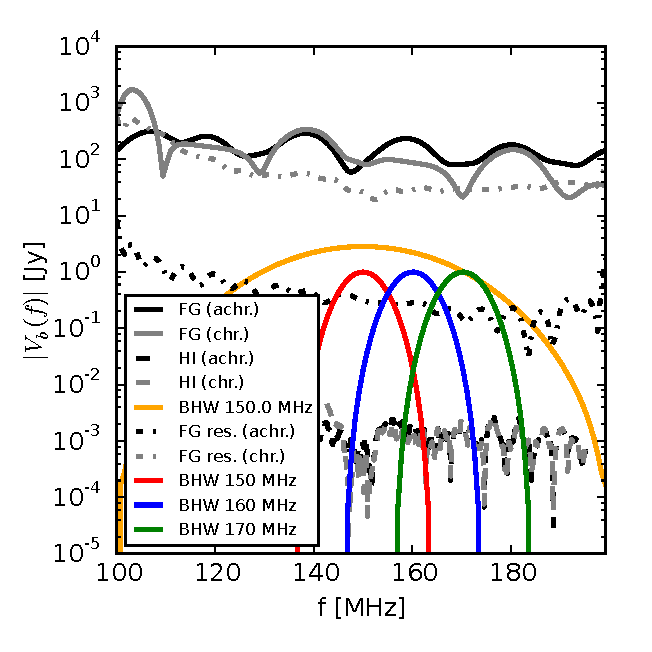
\includegraphics[width=\linewidth]{simulated_FG_EoR_visibilities.eps}
\caption{Simulated EoR H~{\sc i} and foreground visibilities over 100~MHz bandwidth for a 14.6~m baseline of HERA. \label{fig:simulated-visibilities}}
\end{figure}

Figure~\ref{fig:wideband-delay_spectrum} shows the delay spectra of simulated foreground visibilities (in orange) obtained with chromatic (dashed) and achromatic (solid) beams. Neither of them is weighted with the wideband Blackman-Harris window functions in the spectrum. The corresponding CLEAN components are shown in gray and the residuals in black. The depth of deconvolution is set by the limit at which the rms of the residuals inside the horizon limits becomes equal to that on the outside. It is observed that the visibilities simulated with chromatic power pattern (dashed orange) are significantly broadened in delay spectra due to the additional chromaticity. The delay deconvolution is restricted to the {\it foreground wedge} with three additional delay bins on either side of the wedge. Due to this restriction, the residuals inside the horizon delay limits are lower than those outside. Since the simulated visibilities obtained using the achromatic power pattern are predominantly contained well within the horizon delay limits, the delay-domain deconvolution of these delay spectra is much more effective at lowering the residuals (by $\sim 2$ orders of magnitude) than in the case of visibilities obtained with a chromatic power pattern. These delay spectrum residuals correspond to the visibility residuals plotted in Figure~\ref{fig:simulated-visibilities}.

\begin{figure}[htb]
\centering
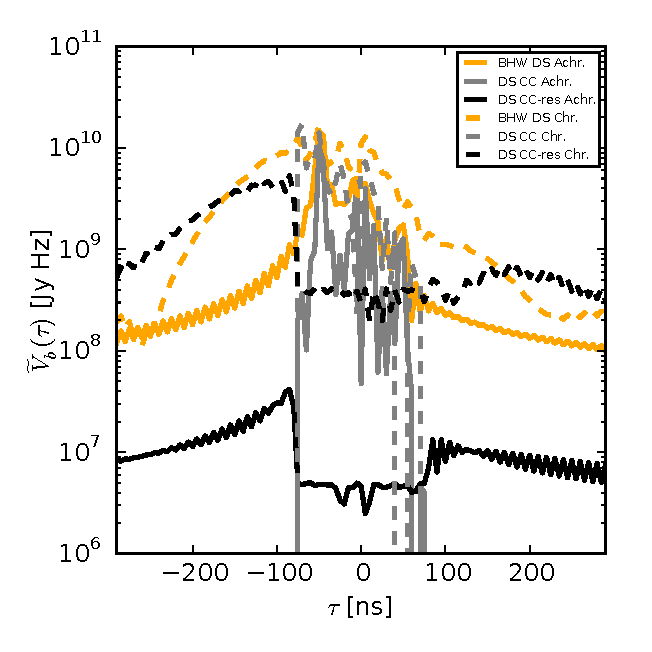
\includegraphics[width=\linewidth]{wideband_simulated_FG_delay_spectrum.eps}
\caption{. \label{fig:wideband-delay_spectrum}}
\end{figure}

Figure~\ref{fig:subband-delay_spectrum} shows the delay spectra of the simulated EoR H~{\sc i} fluctuations and the foregrounds. The three panels show the three different center frequencies (150, 160, and 170~MHz) around which the delay spectra were obtained using the narrow band Blackman-Harris window functions shown earlier in Figure~\ref{fig:simulated-visibilities}. Delay spectra obtained using chromatic and achromatic antenna power patterns are shown in black and gray colors respectively. The dashed lines denote delay spectra of foreground residuals obtained after complex delay-domain deconvolution under the concept of foreground removal. The dotted lines denote the foreground delay spectra obtained under the concept of foreground avoidance where foregrounds were not removed but simply down-weighted by the narrowband Blackman-Harris window unctions.

\begin{figure}[htb]
\centering
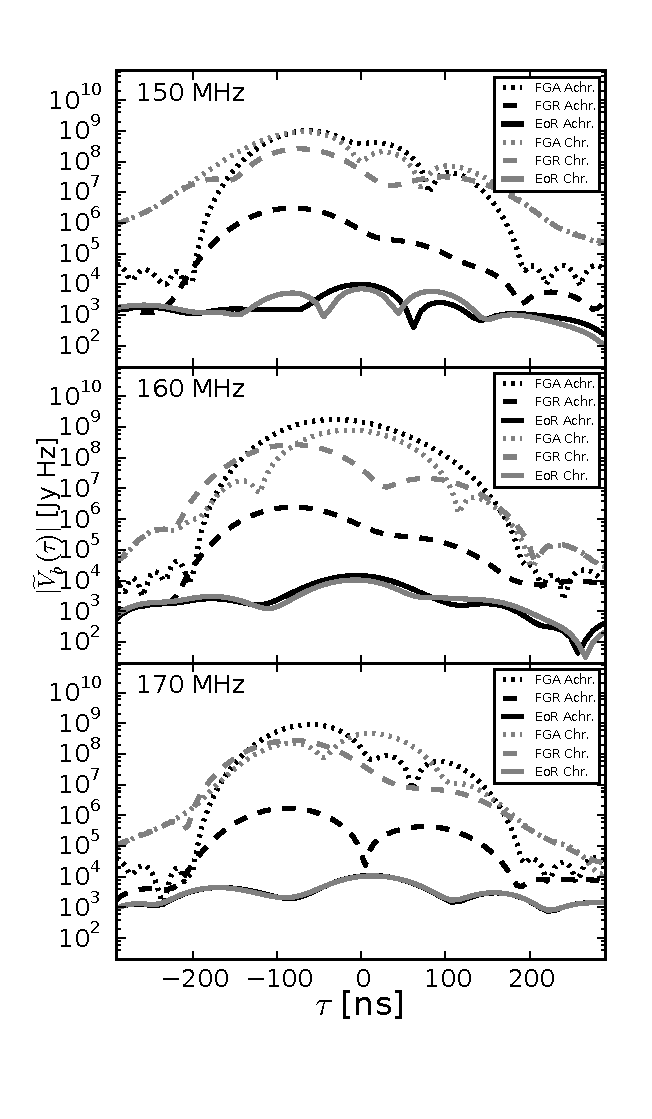
\includegraphics[width=\linewidth]{subband_simulated_EoR_FG_delay_spectrum.eps}
\caption{. \label{fig:subband-delay_spectrum}}
\end{figure}

It is noticed from Figure~\ref{fig:simulated-visibilities} that the foregrounds are about 5 orders of magnitude brighter than the EoR H~{\sc i} fluctuations in the visibilities. From Figure~\ref{fig:subband-delay_spectrum} it is seen that the foreground visibilities under foreground avoidance and their residuals under foreground removal are still brighter than the EoR signal. The delay spectra of foreground residuals however are much closer in magnitude to the EoR signal (to a factor $\lesssim 10$) at $|\tau| \gtrsim 200$~ns.  

\section{Summary}\label{sec:summary}

\acknowledgments

This work was supported by the U. S. National Science Foundation (NSF) through award AST-1109257. DCJ is supported by an NSF Astronomy and Astrophysics Postdoctoral Fellowship under award AST-1401708. JCP is supported by an NSF Astronomy and Astrophysics Fellowship under award AST-1302774. 

% \appendix

% \par\bigskip
\bibliographystyle{apj}
\bibliography{eor}

\end{document}
